\documentclass[conference]{IEEEtran}
\usepackage[T1]{fontenc}
\usepackage{cite}
\usepackage{amsmath,amssymb}
\usepackage{graphicx}
\usepackage{booktabs}
\usepackage{url}
\usepackage[hidelinks]{hyperref}
% Verified final recorded results; dataset SHA-256 7c32b0a358f3257b1cbb3c00e1aea2bdf1a5ac47ea4fff02cdcabedcf9a8fd98
\newcommand{\RawQualitySummary}{Schemas mainly contain INTEGER, TEXT, DATETIME, and REAL attributes. Parsed source statements contain 45,982 explicit NULLs among 1,046,921 literals (4.39\%) and 19,634 omitted column slots, which may receive defaults. There are 60,789 statements with dynamic date expressions, 31 unparsed statements, and 108 column/value mismatches. Only 3,931 of 18,465 table definitions (21.3\%) contain CHECK clauses; constraint coverage is not universal.}
\newcommand{\DatasetSummary}{The benchmark contains 619,619 instances in 999 environments: 127,954 unmodified examples and 491,665 accepted variants (79.35\%). SQLite rejects 38,680 candidates. Date variants account for 75.3\% of positives. The unmodified subset itself exceeds the 100,000-instance requirement.}
\newcommand{\SplitSummary}{Training uses 599 environments (376,201 rows), validation 150 (91,948), and test 250 (151,470).}
\newcommand{\MainSummary}{The test set has 120,137 positives and 31,333 negatives (baseline AP 0.7931). XGBoost has AP 0.9997 and F1 0.9956; differences among ensembles are small. Z-score's validation-selected cutoff predicts every test row positive, giving the same F1 (0.8846) as the constant reference despite better ranking. This shows why F1 alone is insufficient at this prevalence.}
\newcommand{\SeveritySummary}{Each subset has 31,333 negatives and 40,043/40,051/40,043 positives (obvious/medium/subtle), with baseline AP about 0.5610. Isolation Forest AP is 0.7771/0.7612/0.7207; histogram boosting gives 0.9983/0.9982/0.9977.}
\newcommand{\HoldoutSummary}{Omitted dates give AP 0.7410, below the 0.7454 prevalence baseline (91,734 positives), providing no ranking-transfer evidence. Ratings give AP 0.0944 versus baseline 0.0385 (1,253 positives); ages give 0.0053 versus 0.0032 (102 positives). Numeric-type transfer is stronger: money/inventory AP is 0.8861/0.8818 versus baselines 0.3749/0.2085.}
\newcommand{\AblationSummary}{AP is 0.9992, 0.9997, 0.9992; F1 is 0.9924, 0.9955, 0.9939, respectively.}
\newcommand{\RepeatSummary}{AP mean $\pm$ split standard deviation is $0.99728\pm0.00035$ for logistic regression; $0.99951\pm0.00029$ for histogram boosting; $0.89837\pm0.00497$ for Isolation Forest.}
\newcommand{\PrevalenceSummary}{At 1\% (316 positives, 31,333 negatives), histogram boosting AP is 0.9437, but precision is 0.3261 and F1 0.4914. At 5\% (1,649 positives, the same negatives), AP is 0.9857 and precision 0.7157. Fixed-threshold alert quality changes substantially.}
\newcommand{\ShapSummary}{The leading mean absolute attributions are \texttt{min\_year} (0.3474), \texttt{log\_min\_numeric} (0.0486), \texttt{has\_negative\_value} (0.0476). This reflects the controlled date/numeric mutations.}
\newcommand{\ErrorSummary}{RF produces 691 false positives (2.21\% of unmodified test examples) and 594 false negatives (0.49\% of variants). A points redemption of $-1500$ in \texttt{hr\_employee\_management\_1} receives score 1.0 despite being an unmodified debit. In \texttt{ats\_applicant\_tracking\_system\_3}, changing a rating from 4 to 10 receives score 0.005, below the RF threshold 0.2871; the row's identifier 15 leaves its maximum numeric feature unchanged.}
\newcommand{\MainResultsRows}{
Rules & 0.8887 & 0.6723 & 0.9798 \\
Mean/std Z-score & 0.9341 & 0.8846 & 0.7931 \\
Isolation Forest & 0.8964 & 0.8862 & 0.7995 \\
Local Outlier Factor & 0.9509 & 0.8916 & 0.8402 \\
Logistic regression & 0.9977 & 0.9877 & 0.9905 \\
Random Forest & 0.9997 & 0.9947 & 0.9943 \\
Histogram boosting & 0.9992 & 0.9939 & 0.9946 \\
XGBoost & 0.9997 & 0.9956 & 0.9955 \\
Constant reference & 0.7931 & 0.8846 & 0.7931 \\
}


\begin{document}
\title{Mining Silent Data Defects in LLM-Synthesized Agent Environments}
\author{\IEEEauthorblockN{Rahul Jha}
\IEEEauthorblockA{Department of Computer Science\\Texas Christian University\\Fort Worth, Texas, USA\\rahul.jha@tcu.edu}}
\maketitle

\begin{abstract}
Relational databases generated by large language models to train autonomous agents often contain semantic value errors that pass standard database checks without rejection. An employee table might accept an age of 285 or a product table a negative price, because both satisfy the column type constraints. We study whether tabular data mining classifiers can detect these SQL-valid value defects before execution using static query features. Starting with the AgentWorldModel-1K benchmark, we first audited all 129,328 original initialization statements and found 1,374 execution failures across 217 environments, mostly from foreign-key insertion ordering and schema mismatches. One environment had a malformed payload, leaving 999 usable environments. We then generated 491,665 verified silent mutations that execute cleanly in SQLite, pairing them with 127,954 original statements. Across eight detection methods evaluated on disjoint environment partitions, supervised tree ensembles achieved 0.999+ average precision on known corruption patterns. However, holdout tests showed that performance drops to near baseline on omitted defect types (1.1\% recall on dates), and precision fell from 99\% to 32\% when evaluating at 1\% defect prevalence. We interpret feature contributions using TreeExplainer SHAP attributions and present an interactive demonstration for real-time inspection.
\end{abstract}

\section{Problem and Progress Since the Proposal}
Recent reinforcement learning frameworks use language models to synthesize relational databases as training environments for software agents \cite{wang2026awm}. While relational engines enforce data types and primary key constraints, they do not enforce business logic. A transaction with a balance of $-\$500$ or an account opened in the year 1823 executes cleanly in SQLite. Once committed, these silent defects degrade agent policy learning. We evaluate whether lightweight tabular classifiers can detect such SQL-valid defects before statements are executed, without access to the test schemas during training.

Our project proposal outlined a preliminary comparison of simple rules, Isolation Forest, and Random Forest on an in-place sample. Since the proposal, we expanded the work across several dimensions:
\begin{itemize}
    \item Benchmarking eight detection methods across rule-based, unsupervised, and supervised approaches.
    \item Expanding the data into a benchmark of 127,954 original statements and 491,665 separate accepted mutations across 999 usable environments.
    \item Evaluating models under harder conditions, including corruption severity tiers, omitted defect types, cumulative feature groups, random seed splits, and low defect prevalence (1\% and 5\%).
\end{itemize}
Cross-table referential consistency and temporal transaction ordering remain planned for the final project.

\section{Data, Quality, and Leakage Safeguards}
We use the public AgentWorldModel-1K dataset \cite{snowflake2026awm} (CC-BY-4.0), which provides database schemas and seed records for 1,000 synthetic applications.

\textbf{Initialization Audit:} Before generating defects, we tested whether the raw data executes cleanly. Running all 129,328 original INSERT statements in SQLite with foreign keys enabled produced 1,374 failures across 217 environments. Of these, 1,165 were SQLite IntegrityErrors (1,054 foreign-key ordering issues and 111 check or unique constraint violations), and 209 were SQLErrors from malformed syntax or schema mismatches. One environment contained a malformed JSON payload with zero statements. Excluding that environment left 999 usable environments for our benchmark.

\textbf{Defect Injection Pipeline:} We injected four defect types across three severity levels: (1) negative monetary values and quantities (scaled by factors of 10, 1, and 0.1); (2) ratings mutated to 99, 10, or 5.5; (3) ages set to 285, 150, or 120; and (4) dates shifted to 1823, 1950, or offset by $-30$ years. To ensure that every synthetic defect was truly silent, we replayed each candidate statement against a live SQLite instance using transactional savepoints (\texttt{SAVEPOINT} and \texttt{ROLLBACK}). Candidates that triggered any SQLite error were discarded (38,680 rejected candidates). Only statements that executed without database errors were retained. Label 0 denotes an unmodified original statement, and Label 1 denotes an accepted mutation. The resulting dataset contains 619,619 statements (127,954 clean, 491,665 mutations).

\textbf{Environment-Grouped Partitions:} If statements from the same database appear in both training and test sets, models can memorize specific table or column names. To evaluate generalization to unseen applications, we partitioned the data by environment using \texttt{GroupShuffleSplit}. We held out 25\% of environments for testing (250 environments, 151,470 statements) and 20\% of the remainder for validation (150 environments, 91,948 statements), leaving 599 environments (376,201 statements) for training. Scalers and decision thresholds were fitted exclusively on training and validation sets; test labels were never referenced during tuning.

\section{Features, Methods, and Evaluation}
We extracted 26 static numerical features directly from raw SQL statements prior to execution:
\begin{itemize}
    \item \textbf{Value Features (11):} Literal extrema, signed-log min/max numbers, negative value counts, calendar years, flags for years outside 1900--2100, string lengths, and explicit NULL counts.
    \item \textbf{Column-Semantic Features (8):} Keyword matching flags for monetary, inventory, date, age, and rating columns, alongside column and value counts.
    \item \textbf{Schema-Structural Features (7):} Foreign key counts, unique constraints, table width, unknown column counts, query string length, statement index, and fill ratios.
\end{itemize}

\begin{figure}[t]
\centering
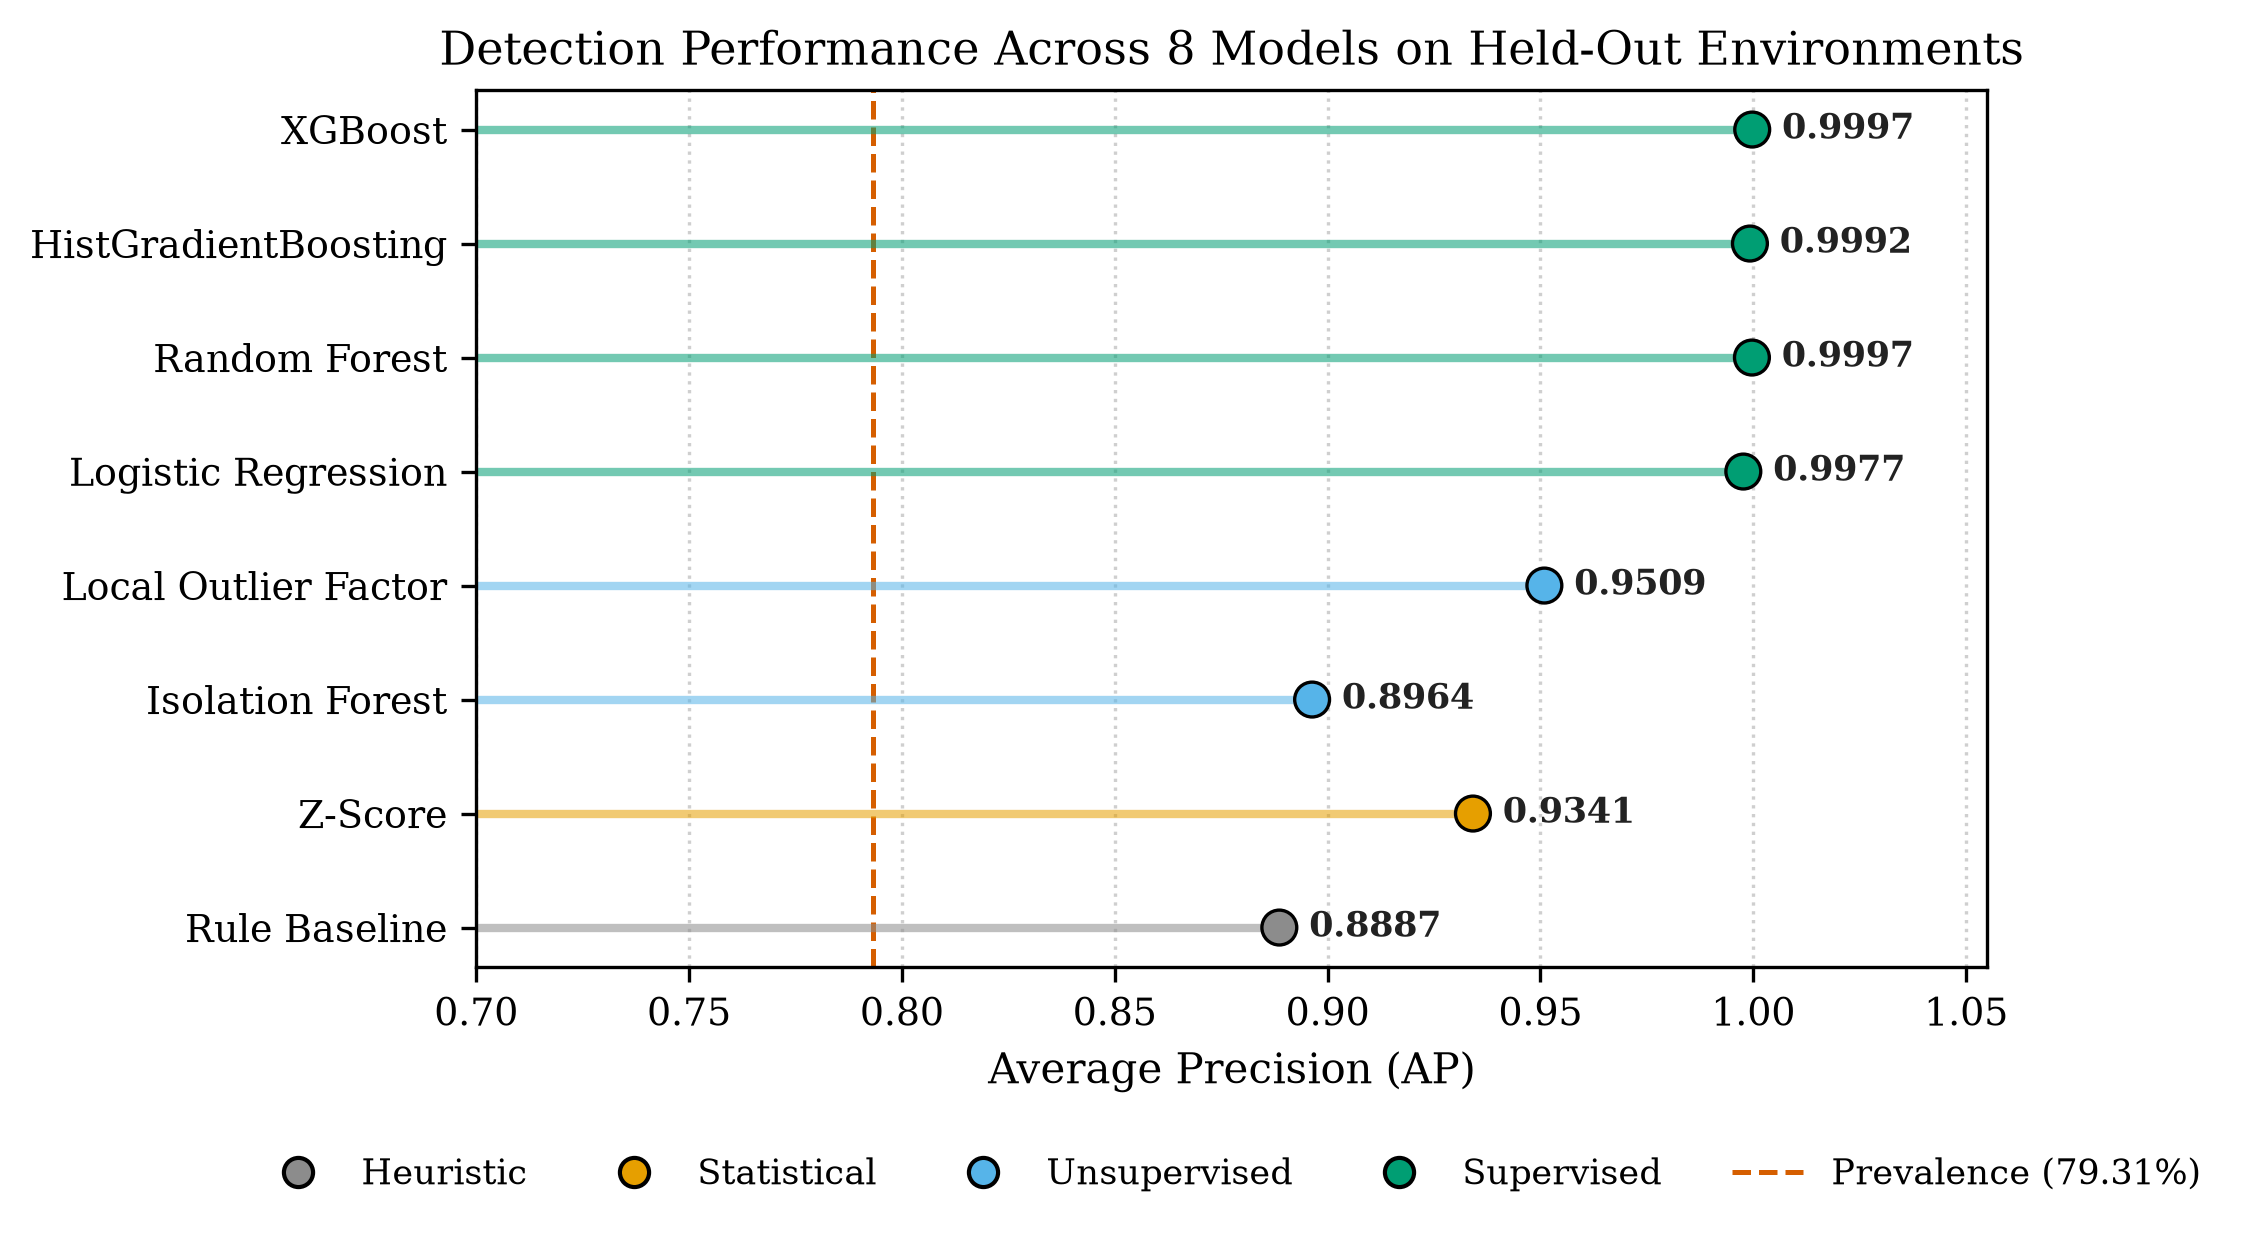
\includegraphics[width=\columnwidth]{figures/fig1_model_comparison.png}
\caption{Detection performance across eight methods on held-out test environments. The dashed line marks the random baseline (79.31\% test prevalence).}
\label{fig:comparison}
\end{figure}

We evaluated eight detection methods:
\begin{itemize}
    \item \textbf{Heuristics:} A rule baseline that flags negative numbers or unusual years when column keywords match, and a Z-score detector that flags rows by maximum standardized feature deviation from clean training records.
    \item \textbf{Unsupervised Outlier Detectors:} Isolation Forest (200 trees) \cite{liu2008isolation} and Local Outlier Factor (LOF, $k=20$, novelty mode) \cite{breunig2000lof}, trained only on unmodified records (Label 0).
    \item \textbf{Supervised Classifiers:} Class-balanced Logistic Regression, Random Forest (200 trees) \cite{breiman2001random}, Histogram Gradient Boosting (max 300 iterations), and XGBoost (300 trees) \cite{chen2016xgboost}.
\end{itemize}
The primary evaluation metric is Average Precision (AP), which corresponds to the area under the Precision-Recall curve. Decision thresholds were chosen on validation data to maximize F1, and Precision@100 measures top-ranked alert accuracy.

\begin{table}[t]
\caption{Held-out test results on 250 unseen environments. Thresholds were selected on validation F1; constant reference predicts all rows positive.}
\label{tab:main}
\centering
\begin{tabular}{lrrr}
\toprule
Method & AP & F1 & Precision \\
\midrule
\MainResultsRows
\bottomrule
\end{tabular}
\end{table}

\section{Experimental Findings and Stress Tests}
Table~\ref{tab:main} and Fig.~\ref{fig:comparison} summarize test performance across the 250 held-out environments.

\textbf{Main Comparison:} In our test split, 79.31\% of statements are mutations (120,137 positive vs. 31,333 negative), meaning a random guess achieves an AP of 0.7931, and predicting all rows positive yields an F1 of 0.8846. Supervised tree models achieved the highest scores: XGBoost reached 0.9997 AP (0.9956 F1), Random Forest reached 0.9997 AP (0.9947 F1), and HistGradientBoosting reached 0.9992 AP (0.9939 F1). Logistic regression reached 0.9977 AP. Unsupervised methods improved upon the random baseline (Isolation Forest 0.8964 AP; LOF 0.9509 AP), but trailed the supervised models. For Z-score, the validation-selected threshold predicted every test instance positive, matching the constant reference F1 (0.8846) despite an AP of 0.9341.

\textbf{Corruption Severity:} Tree ensembles showed consistent ranking performance across severity levels: HistGradientBoosting scored 0.9983 AP on obvious, 0.9982 on medium, and 0.9977 on subtle corruptions. Isolation Forest dropped from 0.7771 on obvious mutations to 0.7207 on subtle ones, indicating that tree isolation depth depends on the numerical magnitude of the shift.

\textbf{Omitted Defect Types:} To evaluate whether models generalize to unseen defect types, we trained models while withholding entire defect families. When dates were omitted from training, test AP on date corruptions fell to 0.7410 (below the 0.7454 prevalence baseline), with a recall of 1.1\%. Omitting ages yielded an AP of 0.0053 against a 0.0032 baseline. In contrast, models trained without inventory corruptions still achieved 0.8818 AP on inventory test cases (baseline 0.2085). This likely reflects shared negative value indicators between inventory and monetary corruptions rather than transfer of domain semantics.

\textbf{Feature Group Ablation:} Evaluating feature subsets with HistGradientBoosting showed that the 11 value features alone achieved 0.9992 AP. Adding column-semantic features yielded 0.9997, and adding schema-structural features yielded 0.9992. Across three random seeds, the standard deviation is $\pm 0.00029$, indicating that literal numeric extrema supply almost all of the discriminative signal.

\textbf{Split Stability and Low Prevalence:} Repeating evaluation across three environment split seeds (42, 43, 44) yielded consistent results ($0.99951 \pm 0.00029$ AP for HistGradientBoosting). However, when we downsampled test mutations to simulate sparse operational settings without retraining, fixed-threshold precision fell to 32.61\% (F1 0.4914) at 1\% prevalence and 71.57\% (F1 0.8284) at 5\% prevalence.

\begin{figure}[t]
\centering
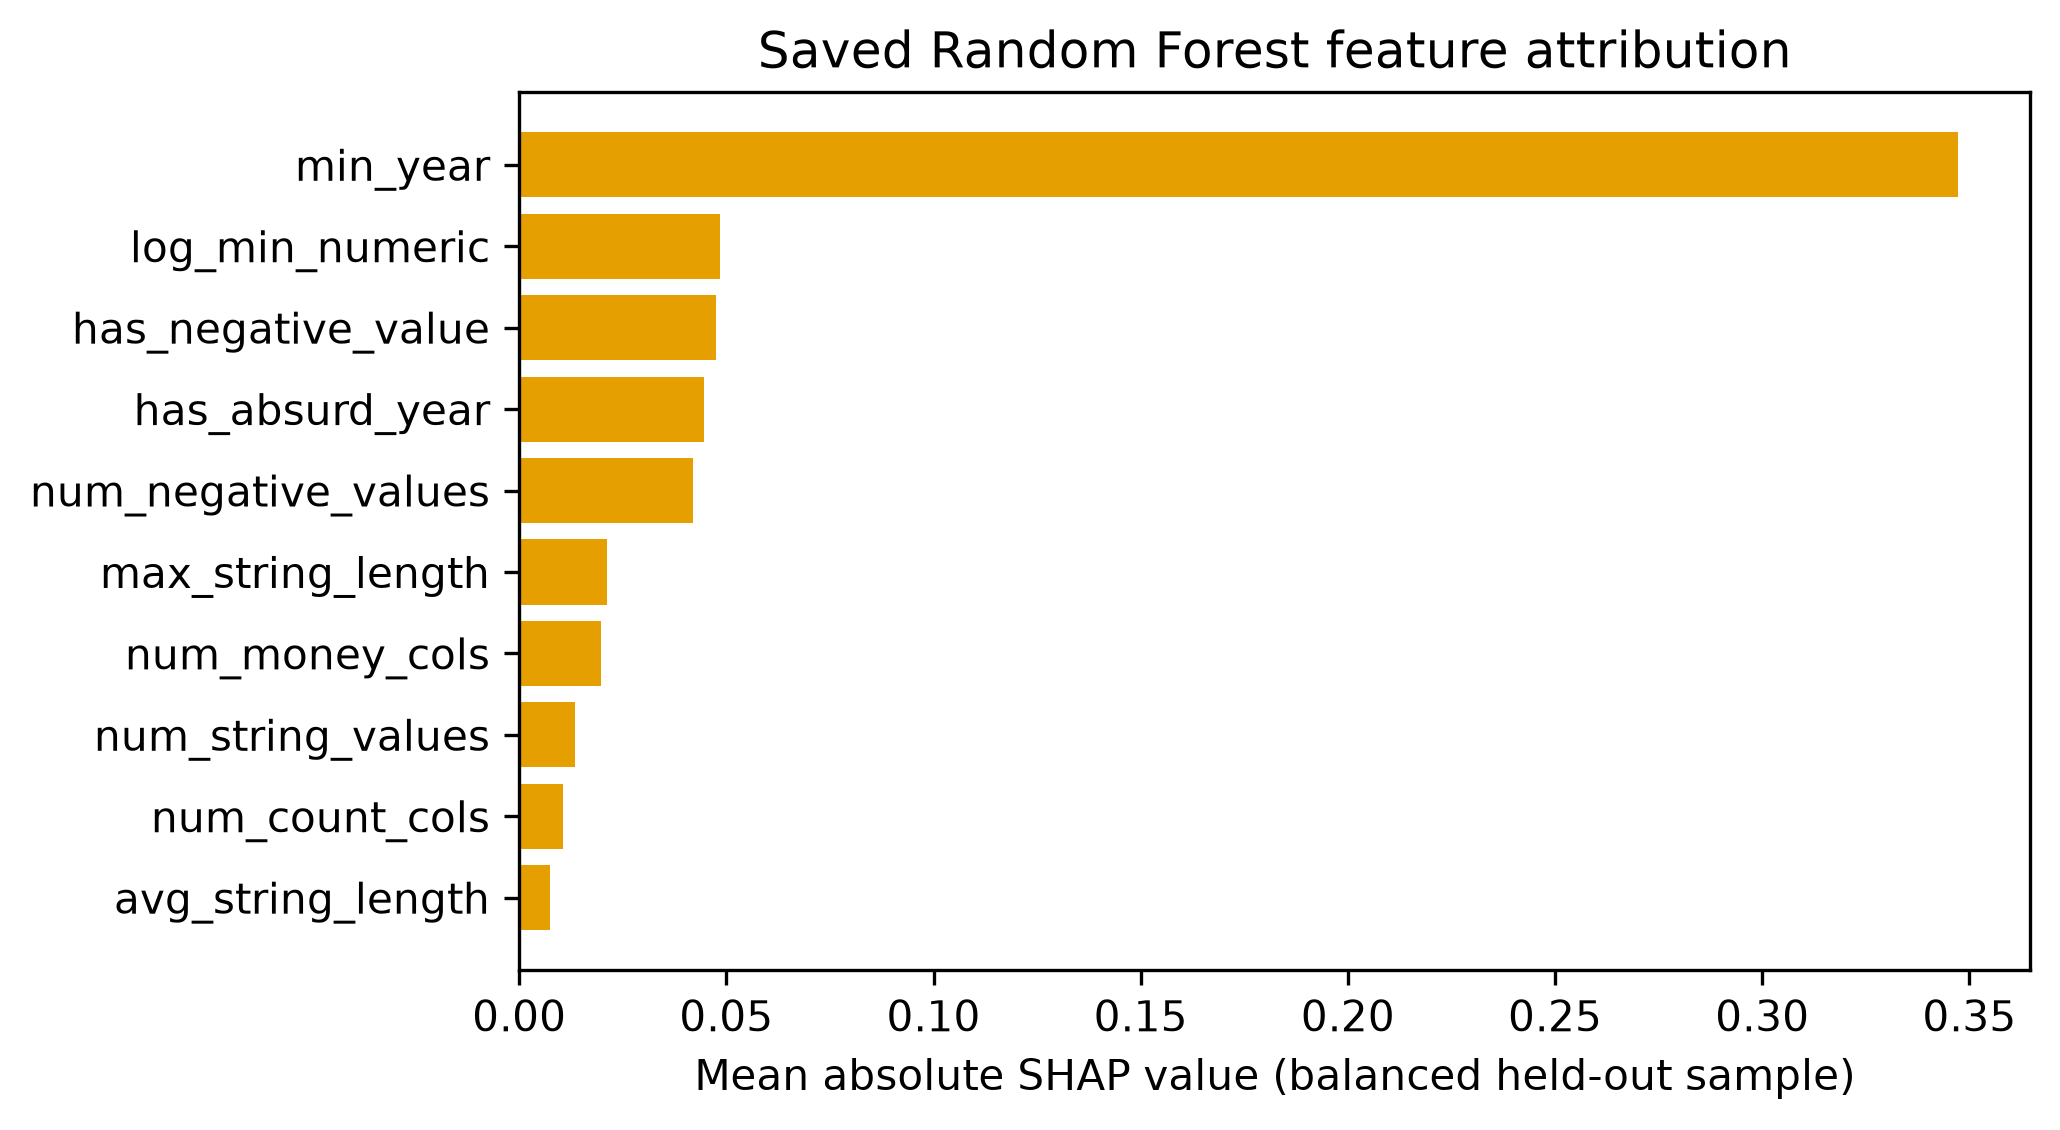
\includegraphics[width=\columnwidth]{figures/fig5_shap_bar.png}
\caption{Mean absolute SHAP values for the Random Forest on a balanced held-out sample, showing the top features driving defect classifications.}
\label{fig:shap}
\end{figure}

\section{Interpretation and Interactive Demonstration}
\textbf{SHAP Feature Attribution:} We analyzed the Random Forest using TreeExplainer SHAP attributions \cite{lundberg2017shap} on a balanced sample of 400 held-out test statements (200 clean, 200 mutations). As shown in Fig.~\ref{fig:shap}, the three largest mean absolute SHAP values were \texttt{min\_year} (0.3474), \texttt{log\_min\_numeric} (0.0486), and \texttt{has\_negative\_value} (0.0476). The attribution for \texttt{min\_year} was more than seven times larger than any other feature, showing substantial reliance on calendar boundaries.

\textbf{Error Case Analysis:} Analyzing misclassifications highlighted the impact of pooling features across entire rows. Random Forest produced 691 false positives (2.21\% of clean test statements) and 594 false negatives (0.49\% of mutations). In an HR database, a legitimate negative points redemption ($-1500$) was assigned a defect probability of 1.0 because the row contained both a negative literal and compensation keywords. In an applicant tracking system, mutating a rating from 4 to 10 produced a score of 0.005 (below the 0.2871 threshold) because an adjacent entity identifier (15) left the row's maximum numeric value unchanged.

\textbf{Interactive Demonstration:} We built a Streamlit application (\texttt{demo\_app.py}) for real-time inspection. Users can enter custom INSERT statements or inspect pre-computed error cases; the application extracts the 26 features, computes model scores, and validates SQLite execution against the corresponding schema. Weights \& Biases tracks experiment runs, metrics, and SHAP artifacts.

\section{Limitations and Future Work}
\begin{itemize}
    \item \textbf{Synthetic Benchmark Bias:} High benchmark accuracy reflects recognition of our specific injection templates. Evaluating real semantic errors requires human domain annotation.
    \item \textbf{Keyword Matching Errors:} Substring matching misclassifies columns, such as matching \texttt{fee} inside \texttt{feels\_like\_c} for temperature, or \texttt{count} inside \texttt{is\_bank\_account}.
    \item \textbf{Row-Wide Feature Masking:} Pooling features across a statement decouples values from their specific column attributes, causing false positives on valid negative numbers.
\end{itemize}
Planned work includes evaluating column-aligned feature representations that bind literals directly to attribute definitions, testing temporal sequence ordering, and auditing cross-table foreign key relationships.

\textbf{Code and Artifacts:} Implementation, tests, and demo are available at \href{https://github.com/jharahul968/awm-silent-defects}{github.com/jharahul968/awm-silent-defects}.

\begin{thebibliography}{8}
\bibitem{wang2026awm} Z. Wang, C. Xu, B. Liu, Y. Wang, S. Han, Z. Yao, H. Yao, and Y. He, ``Agent World Model: Infinity Synthetic Environments for Agentic Reinforcement Learning,'' in \emph{Proc. ICML}, 2026. \url{https://arxiv.org/abs/2602.10090}.
\bibitem{snowflake2026awm} Snowflake AI Research, ``AgentWorldModel-1K,'' 2026. \url{https://huggingface.co/datasets/Snowflake/AgentWorldModel-1K}.
\bibitem{snowflakecode} Snowflake-Labs, ``agent-world-model,'' GitHub repository, 2026. \url{https://github.com/Snowflake-Labs/agent-world-model}.
\bibitem{liu2008isolation} F. T. Liu, K. M. Ting, and Z.-H. Zhou, ``Isolation Forest,'' in \emph{Proc. IEEE ICDM}, 2008, pp. 413--422.
\bibitem{breunig2000lof} M. M. Breunig, H.-P. Kriegel, R. T. Ng, and J. Sander, ``LOF: Identifying Density-Based Local Outliers,'' in \emph{Proc. ACM SIGMOD}, 2000, pp. 93--104.
\bibitem{breiman2001random} L. Breiman, ``Random Forests,'' \emph{Machine Learning}, vol. 45, pp. 5--32, 2001.
\bibitem{chen2016xgboost} T. Chen and C. Guestrin, ``XGBoost: A Scalable Tree Boosting System,'' in \emph{Proc. ACM SIGKDD}, 2016, pp. 785--794.
\bibitem{lundberg2017shap} S. M. Lundberg and S.-I. Lee, ``A Unified Approach to Interpreting Model Predictions,'' in \emph{Advances in Neural Information Processing Systems}, vol. 30, 2017.
\end{thebibliography}
\end{document}
